\documentclass{article}
\usepackage{amsfonts}
\usepackage{graphicx}
\usepackage[margin=1in]{geometry}
\usepackage{bm}
\usepackage{amsmath}
\usepackage{caption}
\usepackage{float}
\renewcommand{\familydefault}{\sfdefault}

\author{Quang P. Nguyen}
\title{Supplementary Materials}
\begin{document}
\maketitle
\captionsetup[figure]{labelfont={bf},name={Figure},labelsep=period, margin=2cm}

\section{Distribution of cILR}
\begin{figure}[h]
    \centering
    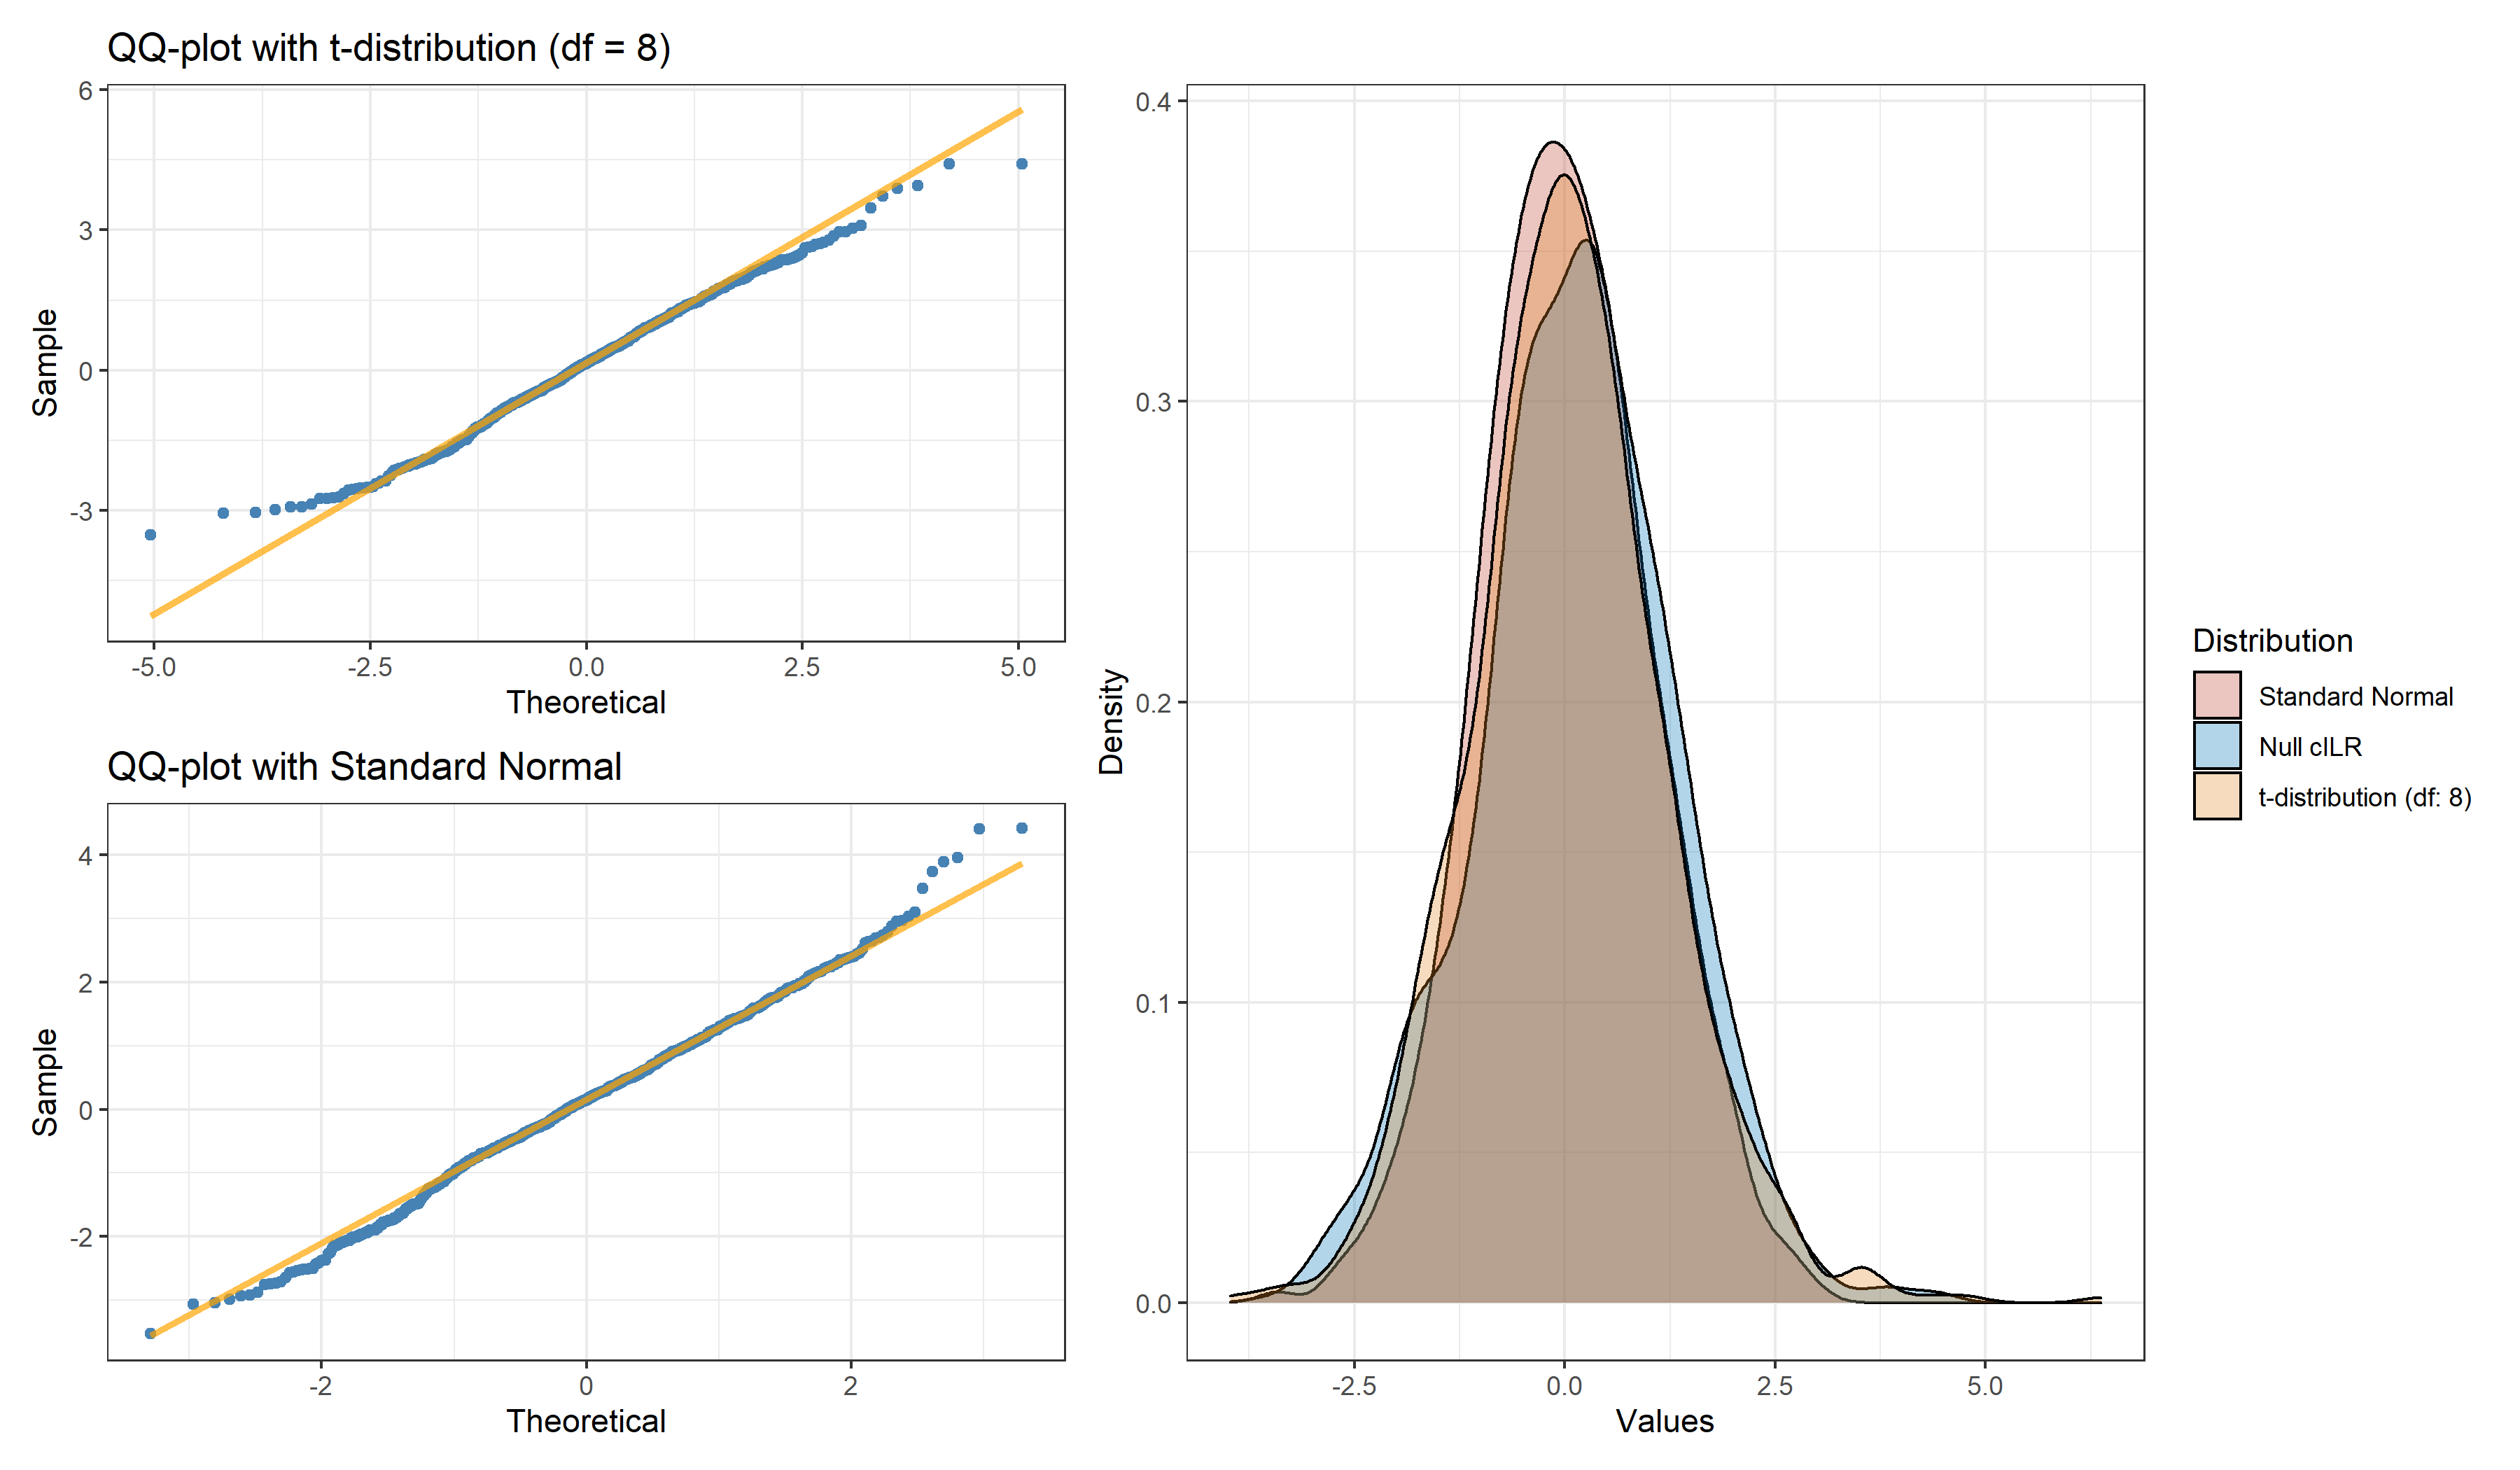
\includegraphics[width=0.8\linewidth]{figures/null_distribution.png}
    \caption{The distribution of cILR statistic under the null. We compared the null distribution of the test statistic and compare it with the standard normal distribution, and the t-distribution with degrees of freedom fitted to cILR scores using the maximum likelihood method}
\end{figure}

\section{Simulation Design}
We simulated microbiome relative abundance data using the Normal to Anything (NorTA) method \cite{cario}. Using this method, we can generate synthetic microbial counts that incorporates a complex correlation structure and multiple types of marginals. The negative binomial distribution was chosen as it has been shown empirically to replicate the overall distribution of real microbiome count data \cite{kurtz2015,calgaro2020}. Parameters used to generate marginal distributions were obtained by fitting non-zero counts of the 16S V3-V5 rRNA stool sequencing data from the human microbiome project (HMP), accquired through via the \emph{HMP16S} package in R \cite{schiffer2019}. In Figure 2, we can see the overall distribution of the fitted mean and size parameter values. \\
To control for overall sparsity, we randomly sample from the count matrix with probability $1 - p_0$ where $p_0$ is the overall desired level of sparsity. Differentially abundant taxa were generated with elevated means with the effect size as the multiplier. We assumed that the overall inter-taxa correlation follows an exchangable structure. \\

\subsection{Hypothesis testing at the sample level}
\noindent For simulations for type I error control, we simulated 100 data sets of 1000 samples each with 1000 taxa per sample with no taxa being significantly enriched. Models were evaluate on a candidate set with varying sizes (50, 100, 150, 200). We also varied the overall sparsity (0.2, 0.4, 0.6, 0.8) and the degree of correlation (0.1, 0.2, 0.5). \\

\noindent For simulations of power and AUC classification capacity, we simulated 100 data sets of 1000 samples each with 1000 taxa per sample with one set of 50 taxa being significantly enriched in either all samples (power evaluation) or half the samples (AUC evaluation). We varied the overall sparsity (0.2, 0.4, 0.8), the correlation (0.1, 0.2, 0.5) and the effect size (2,4,6). \\



\begin{figure}[h]
    \centering
    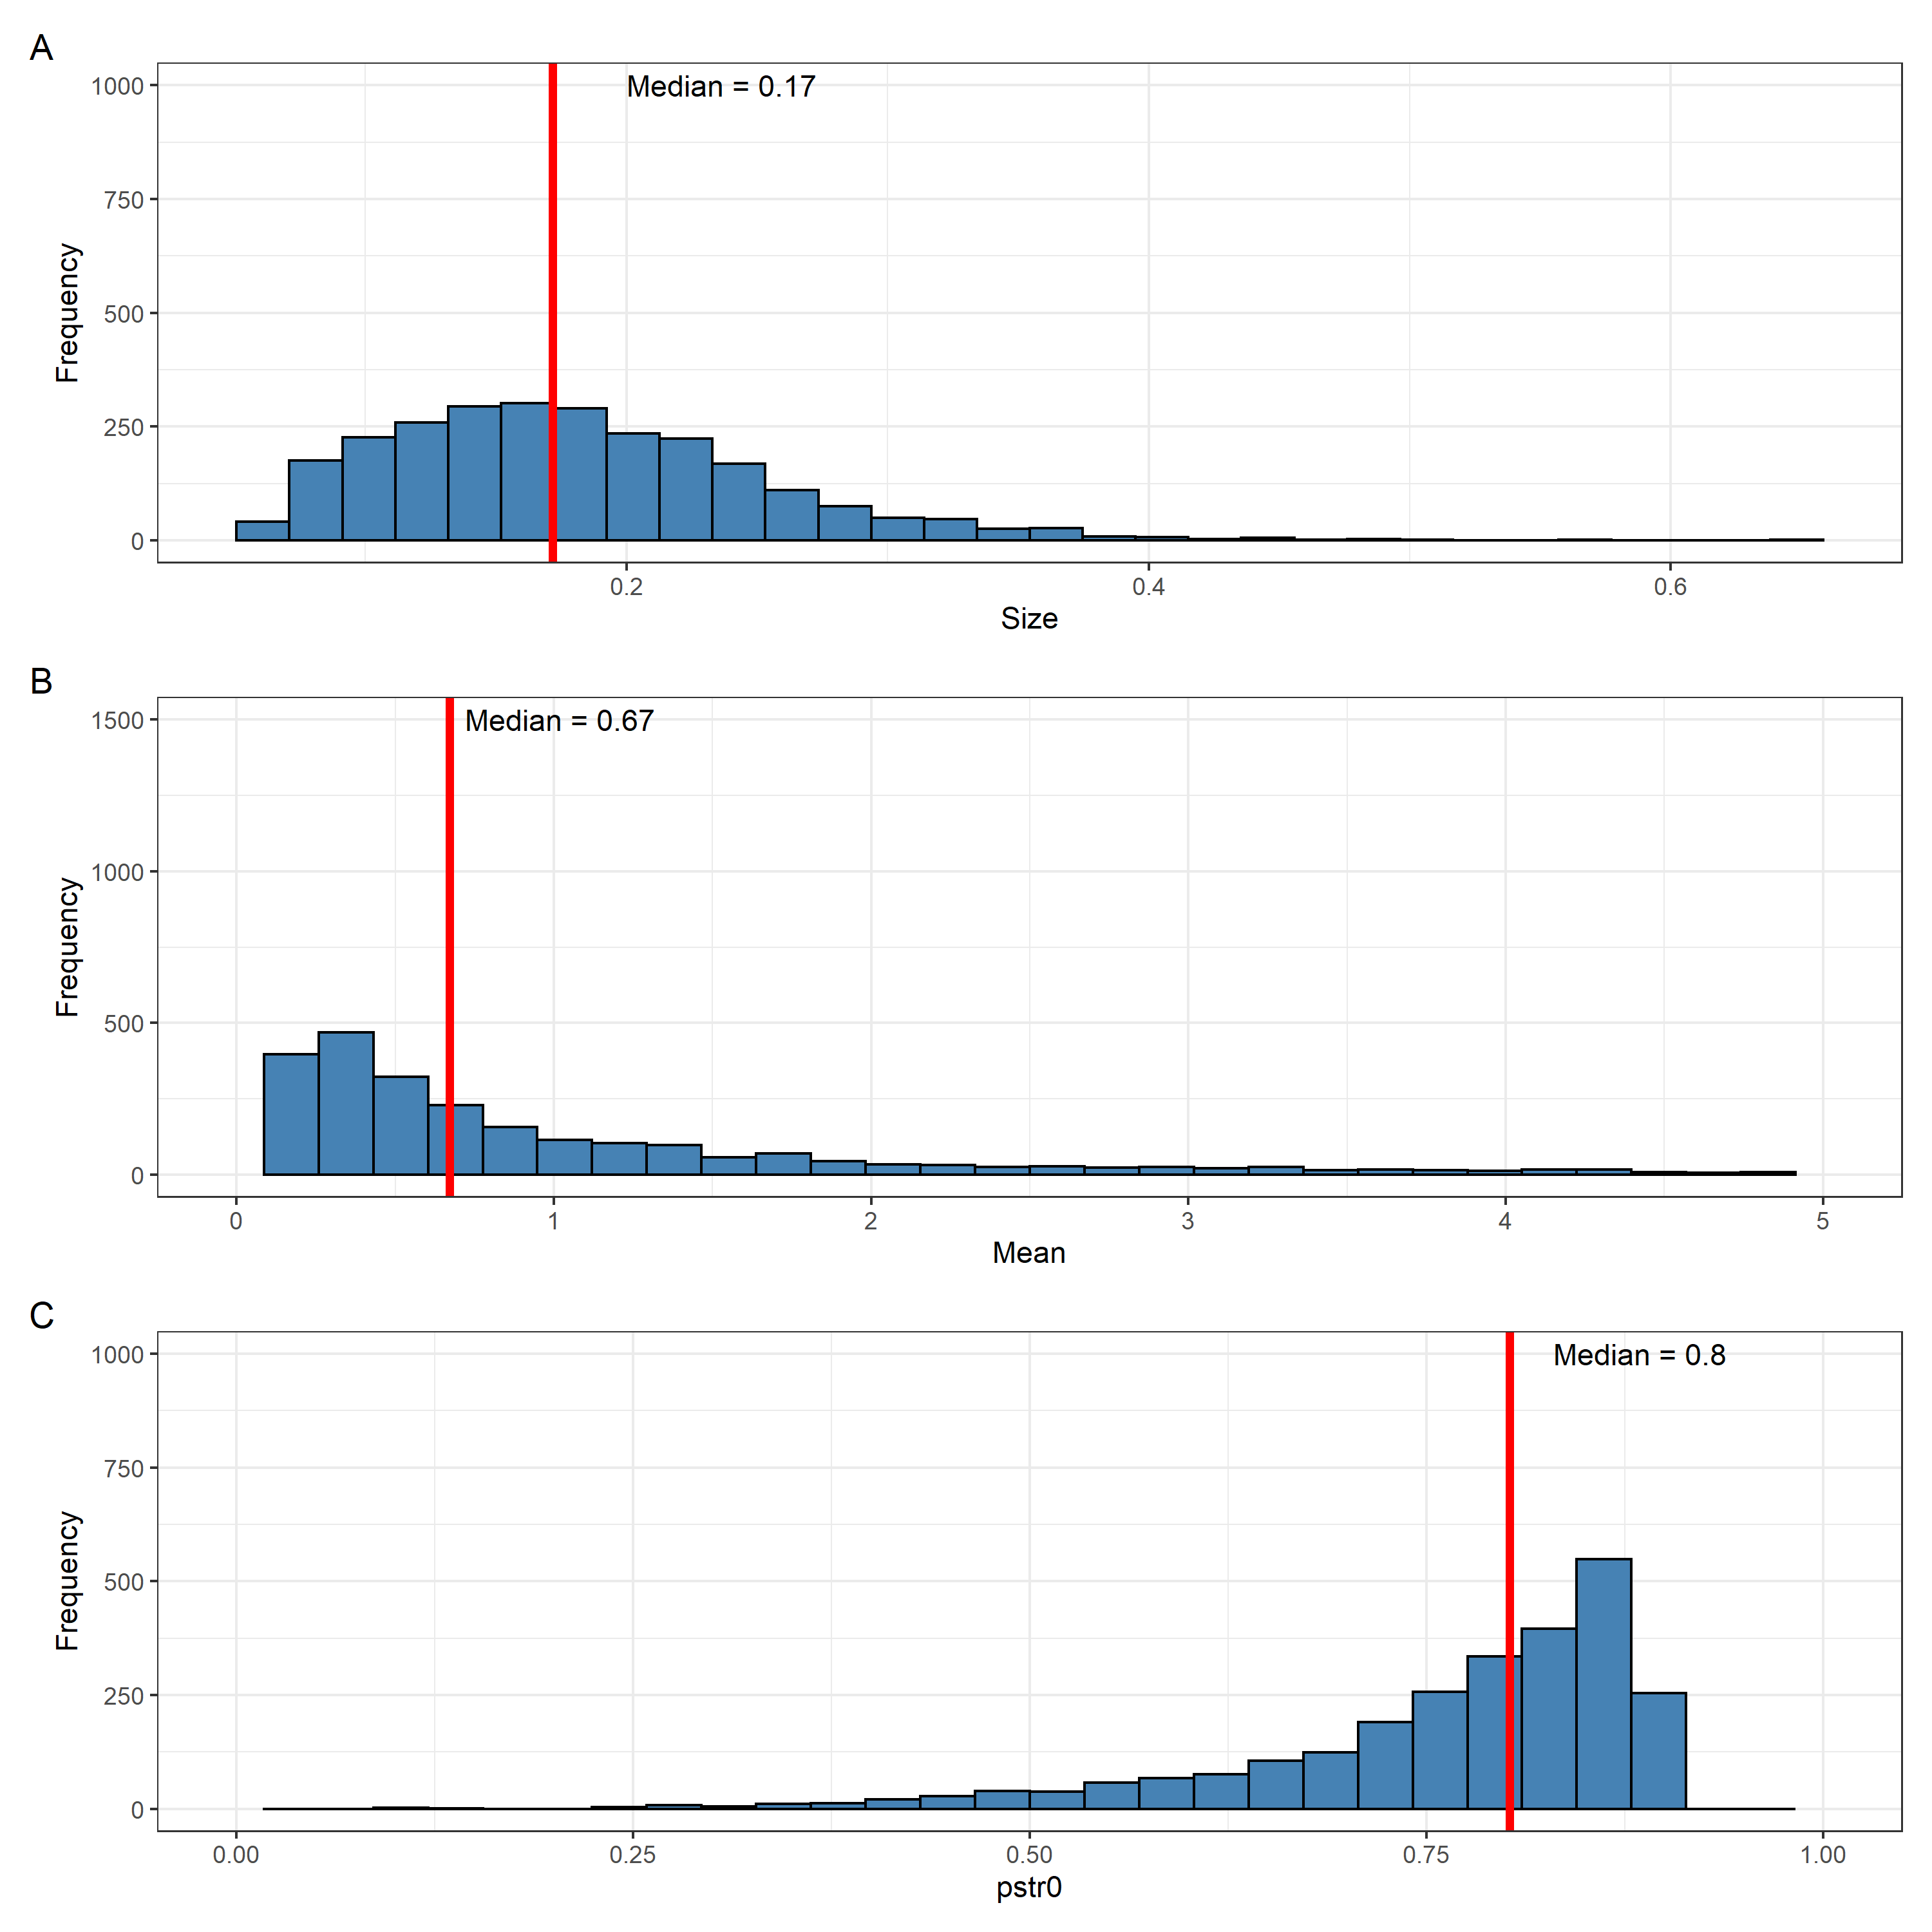
\includegraphics[width=0.6\linewidth]{figures/HMP_fit.png}
    \caption{Distribution of each parameter of the zero inflated negative binomial distribution fitted to \emph{HMP16S} data. The parameters are size (panel A), mean (panel B) and probability of 0 (panel C)}
\end{figure}


\newpage
\bibliography{tax_agg}{}
\bibliographystyle{plain}

\end{document}